% =====================================================================
%  LNCS (Springer Lecture Notes in Computer Science) version.
%
%  Compile with pdfLaTeX. All figures are TikZ/pgfplots, so no image
%  files are needed. Requires the genuine llncs.cls from Springer --
%  Overleaf's "Springer LNCS" template provides it.
% =====================================================================
\documentclass[runningheads]{llncs}

\usepackage[T1]{fontenc}
\usepackage{graphicx}
\usepackage{amsmath,amssymb}
\usepackage{booktabs}
\usepackage{multirow}
\usepackage{rotating}
\usepackage{siunitx}
\usepackage{tikz}
\usepackage{pgfplots}
\usepackage{color}
\usepackage{hyperref}
% Springer's eBook style for URLs (see the LNCS sample file).
\renewcommand\UrlFont{\color{blue}\rmfamily}
\urlstyle{rm}

\pgfplotsset{compat=1.17}
\usetikzlibrary{arrows.meta,positioning,shapes.geometric,fit,backgrounds,calc}
\sisetup{detect-weight=true,detect-family=true}

\definecolor{cData}{HTML}{3B6FA0}
\definecolor{cGen}{HTML}{C06B3E}
\definecolor{cOracle}{HTML}{5B8C5A}
\definecolor{cMuted}{HTML}{8A8A8A}
\definecolor{cRule}{HTML}{D9D9D9}

\begin{document}

\title{Does a Property-Driven Molecular Design Loop Survive Replacing
       its Generator? Swapping G-SchNet for Equivariant Diffusion on
       OE62}
\titlerunning{Swapping G-SchNet for Equivariant Diffusion on OE62}

\author{Jiling Zhong\inst{1} \and Ayan Momin\inst{1}}
\authorrunning{J. Zhong and A. Momin}

\institute{Department of Computer Science, Troy University,
Troy, AL 36082, USA\\
\email{jzhong@troy.edu}, \email{amomin@troy.edu}}

\maketitle

\begin{abstract}
Closed-loop generative design couples a three-dimensional molecular
generator to a property surrogate: molecules are generated, screened,
and the best of them are fed back as training data, so that successive
iterations drift towards a target property. Westermayr et al.\ built
such a loop around G-SchNet, an autoregressive generator, and the OE62
dataset, and reported a chemically interpretable outcome --- cyano
groups became enriched as the electronic gap was driven down. We ask
whether that workflow, and that conclusion, depend on the generator. We
replace G-SchNet with EQGAT-diff, an E(3)-equivariant diffusion model,
holding the dataset and the surrogate architecture fixed so that the
generator is the only variable. The substitution works: the diffusion
generator reaches \SI{97.9}{\percent} atom stability and near-perfect
novelty and uniqueness on OE62, with bond lengths, valencies and
atom-type frequencies close to the training distribution. It also
exposes two costs that the original architecture did not pay. Sampling
is roughly two orders of magnitude more expensive per molecule, so that
a single iteration at the original study's volume would not complete in
a twelve-hour session, and the unconditional property distribution is
about half as wide as the training distribution, so the loop selects
from a narrower band than the data contains. We report the full
selection funnel, which locates the loop's dominant loss in bond
perception on generated coordinates rather than in generation itself, a
two-surrogate agreement filter in place of the original variance check,
and the functional-group enrichment of unbiased samples against OE62.

\keywords{Generative models \and Diffusion models \and Molecular
design \and Equivariant neural networks \and Property optimisation.}
\end{abstract}

% =====================================================================
\section{Introduction}
% =====================================================================

Designing molecules with tailored electronic properties is difficult
because candidate structures must satisfy several competing
requirements at once, and because the space in which they might be
found is far too large to search exhaustively. For organic electronic
materials the requirements are sharp: the fundamental gap, the
ionisation potential and the electron affinity must each fall inside a
narrow window for a device to function at
all~\cite{westermayr2022,stuke2020}. Which structural changes move
those quantities in the right direction is rarely obvious in advance,
so candidate identification still rests largely on chemical intuition
and trial and error.

Generative deep learning has emerged as a route past that bottleneck.
Models that predict three-dimensional conformations directly are
particularly attractive here, because the atomic configuration is what
electronic-structure methods --- and the machine learning models that
approximate them --- take as input. But a generator trained on a
structural distribution reproduces that distribution: it will satisfy
the learned chemical rules, and will possess specific target properties
only by chance. Unguided sampling is therefore an inefficient way to
reach a narrow property window, particularly when the window sits in
the tail of the training distribution.

The established remedy is to close the loop. Westermayr et
al.~\cite{westermayr2022} generate in bulk with
G-SchNet~\cite{gebauer2019}, screen the output with a fast property
surrogate, retain the extreme tail, retrain the generator on that tail,
and repeat --- driving the fundamental gap, the ionisation potential
and the electron affinity beyond the ranges present in OE62. Their most
striking result was not a number but a chemical pattern: molecules
selected for small gaps were enriched in cyano
($\mathrm{C}\!\equiv\!\mathrm{N}$) groups, and a knock-out experiment,
in which every C$\equiv$N bond was removed from the training set before
retraining, confirmed the association.

That pattern is attributed to the chemistry. It was, however, obtained
with a single generator, and generators differ in ways that could
plausibly shape which regions of chemical space a loop explores.
G-SchNet places atoms sequentially, conditioned on what it has already
placed, and emits coordinates only. Diffusion models such as
EQGAT-diff~\cite{le2023} instead denoise all atoms simultaneously under
an equivariance constraint, and jointly model discrete atom and bond
types alongside continuous coordinates. Nothing guarantees that two
such different samplers, trained on the same data and steered by the
same surrogate, discover the same chemistry --- or that a protocol
tuned for one of them transfers to the other at all.

\subsubsection{Contribution.} In this work we substitute EQGAT-diff for
G-SchNet inside the loop of~\cite{westermayr2022}, holding the dataset
and the surrogate architecture fixed so that the generator is the only
variable, and report:

\begin{enumerate}
  \item A reproducible OE62 preparation pipeline for a bond-aware
        generator, including the cost of inferring bonds for a dataset
        that stores none, and the element coverage that cost imposes
        (Section~\ref{sec:data}).
  \item Unconditional generation quality for the diffusion generator on
        OE62, with binomial confidence intervals and the failure profile
        that limits validity on a twelve-element alphabet
        (Section~\ref{sec:uncond}).
  \item The full selection funnel of one biasing iteration, which
        locates the loop's dominant loss in bond perception on generated
        coordinates rather than in generation (Section~\ref{sec:funnel}).
  \item Two measured costs of the substitution --- sampling throughput
        and the width of the unconditional property distribution ---
        which together determine whether the original protocol is
        reachable with a diffusion generator at all
        (Section~\ref{sec:discussion}).
\end{enumerate}

% =====================================================================
\section{Related Work}
% =====================================================================

\subsubsection{Three-dimensional molecular generation.}
Early generative models of molecules operated on SMILES strings or
molecular graphs, which fix connectivity but not geometry; a
three-dimensional conformation then has to be produced by a separate
embedding step, and need not correspond to an energetic
minimum~\cite{westermayr2022}. G-SchNet~\cite{gebauer2019} instead
generates 3D point sets directly, placing atoms one at a time using
rotationally invariant features derived from SchNet~\cite{schutt2018},
so the output is already close to a relaxed geometry. Diffusion models
followed, learning to invert a noising process over coordinates;
EQGAT-diff~\cite{le2023} is among the strongest of these and differs
from earlier diffusion generators in modelling discrete atom and bond
types jointly with continuous coordinates, under an $x_0$-parameterised
objective.

\subsubsection{Property-driven generation.}
Making a generator produce molecules with target properties, rather
than merely plausible ones, is approached in three broad ways:
conditioning the generator on the property at training
time; steering sampling with gradients from a differentiable predictor;
or leaving the generator unconditional and closing a loop around it by
screening and retraining. The last is the approach
of~\cite{westermayr2022} and the one we study, because it treats the
generator as a replaceable component --- which is precisely what makes
the substitution question well posed.

\subsubsection{Bond perception.}
Converting a set of atomic coordinates into a bonded molecule is a
classical problem, solved in practice by distance-based connectivity
followed by a combinatorial search over bond orders subject to valence
constraints~\cite{kim2015}. The procedure is reliable on equilibrium
geometries and degrades on distorted ones, which matters here because
generated structures are not relaxed. Section~\ref{sec:funnel}
quantifies that degradation for our pipeline.

% =====================================================================
\section{Methods}
% =====================================================================

\subsection{Data preparation}
\label{sec:data}

EQGAT-diff models bond types explicitly, so OE62's coordinate-only
structures must be given bonds before training. We infer them with
RDKit's \texttt{rdDetermineBonds}, a combinatorial bond-order search.
Two practical issues arise at this scale.

First, the search has no internal time limit and diverges on certain
molecules. We measured a median perception time below
\SI{10}{\milli\second}, but a small number of molecules did not
terminate within an hour. We therefore run perception in a pool of
killable worker processes with a per-molecule timeout of
\SI{5}{\second}. Exactly \num{55} molecules (\SI{0.09}{\percent}) hit
the timeout; all were polynitro or polysulfur species between 26 and 70
atoms, with no dependence on size.

Second, perception fails outright on \num{3067} molecules
(\SI{5.3}{\percent} of those passing the size gate, \SI{5.0}{\percent} of all released structures). This failure is not uniform across the periodic
table: it removes \emph{every} molecule containing Se, As, Te or Li
($\approx$\num{1082} molecules), so the generator sees
\textbf{12 of OE62's 16 elements}. We regard this as a property of the
preparation step rather than of the generator, and state it as a scope
restriction.

We cap molecules at 70 atoms, removing \num{3795} structures.
\cite{westermayr2022} train on the full OE62 size range but restrict
their IP-biasing experiment to molecules of at most 70 atoms for the
same tractability reason; we apply the cap throughout. Table~\ref{tab:funnel-data} gives the full
accounting. The pipeline is deterministic up to worker scheduling: three
runs on two machines produced \num{54570}, \num{54572} and \num{54575}
molecules, a spread below \SI{0.01}{\percent}. We use a
\num{80}/\num{10}/\num{10} split, giving $\approx$\num{43657} training
molecules.

\begin{table}[t]
\centering
\caption{OE62 preparation. Percentages are of the \num{61489} released
structures.}
\label{tab:funnel-data}
\begin{tabular}{lrr}
\toprule
Stage & Molecules & Share \\
\midrule
Released structures            & \num{61489} & \SI{100.0}{\percent} \\
Removed, $>70$ atoms           & \num{-3795} & \SI{6.2}{\percent} \\
Passing size and element gates & \num{57694} & \SI{93.8}{\percent} \\
Removed, bond perception failed& \num{-3067} & \SI{5.0}{\percent} \\
Removed, perception timeout    & \num{-55}   & \SI{0.09}{\percent} \\
\midrule
\textbf{Training corpus}       & \textbf{\num{54572}} & \SI{88.8}{\percent} \\
\bottomrule
\end{tabular}
\end{table}

\subsection{Generator}

We train EQGAT-diff with the authors' default architecture
(\num{824000} parameters; scalar dimension 128, vector dimension 32,
six layers) for 100 epochs on a single NVIDIA T4, which took
\SI{7}{\hour}\,\SI{5}{\minute} at \SI{4}{\minute}\,\SI{8}{\second} per
epoch. No pretraining or transfer learning is used.

\subsection{Property surrogate}

The target is the HOMO--LUMO gap as stored in OE62. We train a
SchNet-style regressor (\num{455809} parameters) on atomic numbers and
coordinates only --- the surrogate never sees a bond, which matters in
Section~\ref{sec:funnel}. Of the \num{57694} molecules passing the size
and element gates, all carry a gap label, giving a
\num{51925}/\num{5769} train/validation split with target
$\mu=\SI{5.10}{\electronvolt}$, $\sigma=\SI{1.03}{\electronvolt}$.

Two surrogates are trained with different seeds, implementing the
two-model reliability check of~\cite{westermayr2022}. They reach
validation MAEs of \SI{0.2262}{\electronvolt} and
\SI{0.2330}{\electronvolt}; a third training of the same configuration
gave \SI{0.2373}{\electronvolt}, so run-to-run spread is
$\approx$\SI{0.004}{\electronvolt}. For reference, a predictor that always returns the mean would score
$\sigma\sqrt{2/\pi}\approx\SI{0.82}{\electronvolt}$, and
\cite{westermayr2022} report $\approx$\SI{0.25}{\electronvolt} for their
surrogate. During screening, a molecule is discarded when the two
predictions differ by more than the sum of their validation MAEs
(\SI{0.4593}{\electronvolt}); survivors are scored with the mean of the
two. \cite{westermayr2022} discard when the disagreement exceeds the
\emph{average} of the two errors rather than their sum, a threshold twice
as strict; we report results under the looser criterion and note the
difference.

Figure~\ref{fig:oracle} shows the learning curves. Both surrogates
overfit substantially --- final training error is roughly an order of
magnitude below validation error --- which we return to in
Section~\ref{sec:discussion}.

% ---------------------------------------------------------------------
\begin{figure}[t]
\centering
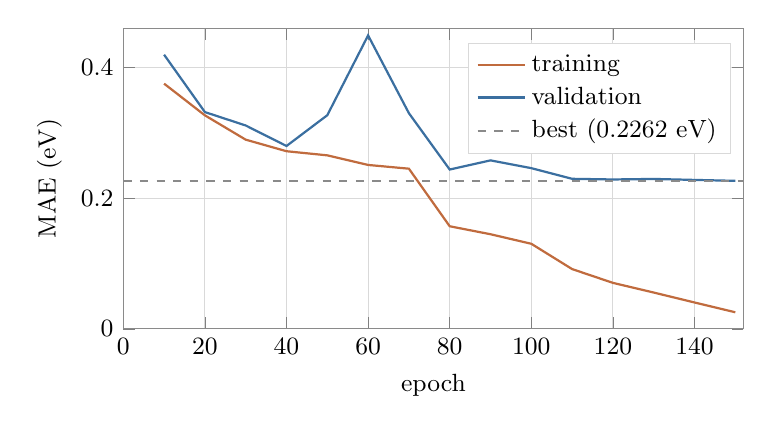
\begin{tikzpicture}
\begin{axis}[
  width=0.78\linewidth, height=5.4cm,
  xlabel={epoch}, ylabel={MAE (eV)},
  xmin=0, xmax=152, ymin=0, ymax=0.46,
  grid=major, grid style={cRule},
  axis line style={cMuted}, tick label style={font=\small},
  label style={font=\small},
  legend style={font=\small,draw=cRule,at={(0.98,0.95)},anchor=north east},
  legend cell align=left,
]
\addplot[cGen,thick,mark=none] coordinates {
 (10,0.3752)(20,0.3267)(30,0.2895)(40,0.2718)(50,0.2655)(60,0.2508)
 (70,0.2451)(80,0.1570)(90,0.1448)(100,0.1302)(110,0.0915)(120,0.0704)
 (130,0.0556)(140,0.0404)(150,0.0254)};
\addlegendentry{training}
\addplot[cData,thick,mark=none] coordinates {
 (10,0.4195)(20,0.3317)(30,0.3112)(40,0.2798)(50,0.3269)(60,0.4490)
 (70,0.3300)(80,0.2438)(90,0.2578)(100,0.2459)(110,0.2296)(120,0.2286)
 (130,0.2294)(140,0.2279)(150,0.2265)};
\addlegendentry{validation}
\addplot[cMuted,dashed,thick,mark=none] coordinates {(0,0.2262)(152,0.2262)};
\addlegendentry{best (0.2262 eV)}
\end{axis}
\end{tikzpicture}
\caption{Surrogate learning curves. Validation error plateaus by epoch
$\approx$110 while training error keeps falling to
\SI{0.0254}{\electronvolt}, a ratio of \num{8.9}. The saved checkpoint is
the best-validation one, so the overfitting costs compute rather than
accuracy --- but it is a warning about predictions on off-distribution
inputs.}
\label{fig:oracle}
\end{figure}
% ---------------------------------------------------------------------

\subsection{Loop configuration}

Table~\ref{tab:config} lists the settings used for the iteration
reported in Section~\ref{sec:funnel}. Sampling uses \num{500} denoising
steps per molecule, the EQGAT-diff default, in batches of \num{20}
graphs.

\begin{table}[t]
\centering
\caption{Loop configuration. The agreement threshold is the sum of the
two surrogates' validation MAEs, computed at run time rather than fixed
in advance.}
\label{tab:config}
\begin{tabular}{lll}
\toprule
Stage & Setting & Value \\
\midrule
\multirow{2}{*}{Generation}
 & molecules per iteration        & \num{3000} \\
 & denoising steps, batch size    & \num{500}, \num{20} \\
\midrule
\multirow{2}{*}{Screening}
 & perception charges tried       & $0,\pm1,\pm2$ \\
 & agreement threshold            & \SI{0.4593}{\electronvolt} \\
\midrule
\multirow{3}{*}{Selection}
 & target, direction              & HOMO--LUMO gap, minimise \\
 & threshold                      & $\mu-0.5\sigma$ \\
 & minimum to proceed             & \num{20} molecules \\
\midrule
Fine-tuning
 & learning rate                  & $1\times10^{-4}$ \\
\bottomrule
\end{tabular}
\end{table}

\subsection{Screening and selection}

Generated structures are written as coordinates, so bonds must be
inferred a second time. We perceive in two stages. Connectivity alone
(\texttt{DetermineConnectivity}) is enough to reject fragmented
structures and enough for the surrogate, which reads only atomic
numbers and positions. Full bond orders
(\texttt{DetermineBonds}) are required only to write a training file for
fine-tuning, and are attempted at net charges
$\{0,\pm1,\pm2\}$: insisting on neutrality discards every generated ion,
which in our measurements removed the majority of otherwise usable
samples. Selection keeps molecules below $\mu - 0.5\sigma$ of the
predicted gap distribution.

% =====================================================================
\section{Results}
% =====================================================================

\subsection{Unconditional generation}
\label{sec:uncond}

Table~\ref{tab:uncond} reports standard metrics on the \num{3000}
samples drawn from the 100-epoch model at iteration~0. These are the
same structures that Table~\ref{tab:funnel-loop} follows through the
screening stages, so every figure in this section describes one
generation run rather than several.

\begin{table}[t]
\centering
\caption{Unconditional generation quality: \num{3000} samples from the
100-epoch model, the same batch that Table~\ref{tab:funnel-loop} follows
through the loop. Intervals are \SI{95}{\percent} Wilson bounds on the
binomial proportion. W1 and TV entries are distances between the generated
and training distributions, so lower is better.}
\label{tab:uncond}
\begin{tabular}{llr@{\hspace{1em}}l}
\toprule
 & Metric & Value & \SI{95}{\percent} CI \\
\midrule
\multirow{4}{*}{\rotatebox[origin=c]{90}{\footnotesize validity}}
 & validity                      & \SI{23.9}{\percent} & [22.4, 25.5] \\
 & sanitisation validity          & \SI{29.6}{\percent} & \\
 & molecule stability             & \SI{51.9}{\percent} & [50.1, 53.7] \\
 & atom stability                 & \SI{97.9}{\percent} & [97.8, 98.0] \\
\midrule
\multirow{3}{*}{\rotatebox[origin=c]{90}{\footnotesize variety}}
 & novelty                        & 0.996 & \\
 & uniqueness                     & 1.000 & \\
 & diversity                      & 0.819 & \\
\midrule
\multirow{7}{*}{\rotatebox[origin=c]{90}{\footnotesize distribution}}
 & ChargeW1 $\downarrow$          & 0.002 & \\
 & BondLengthsW1 $\downarrow$     & 0.020 & \\
 & EdgeTypesTV $\downarrow$       & 0.025 & \\
 & ValencyW1 $\downarrow$         & 0.030 & \\
 & AtomTypesTV $\downarrow$       & 0.036 & \\
 & NumNodesW1 $\downarrow$        & 0.541 & \\
 & AnglesW1 $\downarrow$          & 6.65 & \\
\midrule
 & connected components (mean)    & 1.29 & \\
\bottomrule
\end{tabular}
\end{table}

Three observations. First, atom stability of \SI{97.9}{\percent}
(\SI{95}{\percent} CI \SIrange{97.8}{98.0}{\percent} over \num{116400}
atoms) and small distributional distances on charges, bond lengths, bond
types and valencies indicate that local chemistry is learned well: the
model places the right atoms at the right distances with the right formal
charges.

Second, novelty of \num{0.996} with uniqueness of \num{1.000} means a
handful of generated molecules reproduce an OE62 entry and none repeats
another, so there is neither substantial memorisation nor mode collapse.

Third, molecule-level validity of \SI{23.9}{\percent}
(\SIrange{22.4}{25.5}{\percent}) is low in absolute terms, and the failure
profile locates the reason. Of \num{3000} samples, \num{718} pass; among
the reported failures, atom valence (\num{781}) and kekulisation
(\num{671}) dominate, against \num{93} of other kinds. Both are
combinatorial in the size of the element alphabet: with twelve elements
there are far more ways to assign a valence that no bond-order assignment
can satisfy than with the four of a CHNO-restricted problem.

The gap between atom and molecule stability is informative in its own
right. If atoms failed independently, a molecule of the mean size
(\num{38.8} atoms) would be stable with probability
$0.979^{38.8}=\num{0.436}$, whereas \SI{51.9}{\percent} are observed.
Unstable atoms therefore cluster within molecules rather than scattering
across them --- the model does not degrade uniformly, it produces mostly
clean molecules alongside a minority that are locally wrong in several
places at once.

\subsection{The selection funnel}
\label{sec:funnel}

Table~\ref{tab:funnel-loop} and Figure~\ref{fig:funnel} trace one
iteration from \num{3000} generated structures to \num{74} selected
molecules.

\begin{table}[t]
\centering
\caption{One biasing iteration, starting from the unbiased 100-epoch
model. ``Share'' is of the \num{3000} structures generated.}
\label{tab:funnel-loop}
\begin{tabular}{lrrl}
\toprule
Stage & Count & Share & Limited by \\
\midrule
Generated                & \num{3000} & \SI{100}{\percent} & --- \\
Written to disk          & \num{1557} & \SI{51.9}{\percent} & molecule stability \\
Single connected component& \num{261} & \SI{8.7}{\percent}  & bond perception \\
Surviving agreement filter& \num{241} & \SI{8.0}{\percent}  & surrogate disagreement \\
\textbf{Selected} ($\mu-0.5\sigma$) & \textbf{\num{74}} & \SI{2.5}{\percent} & selection threshold \\
\bottomrule
\end{tabular}
\end{table}

% ---------------------------------------------------------------------
\begin{figure}[t]
\centering
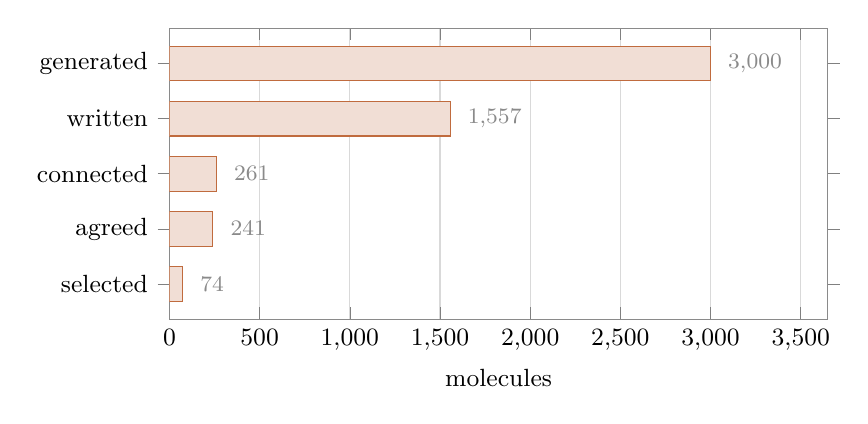
\begin{tikzpicture}
\begin{axis}[
  width=0.82\linewidth, height=4.6cm,
  xbar, y=7mm, bar width=4.4mm,
  xmin=0, xmax=3650,
  xlabel={molecules}, label style={font=\small},
  symbolic y coords={selected,agreed,connected,written,generated},
  ytick=data, yticklabel style={font=\small},
  nodes near coords, nodes near coords style={font=\footnotesize,text=cMuted},
  every node near coord/.append style={xshift=1mm},
  axis line style={cMuted}, tick label style={font=\small},
  xmajorgrids, grid style={cRule},
  enlarge y limits=0.16,
]
\addplot[draw=cGen,fill=cGen!22] coordinates {
  (3000,generated) (1557,written) (261,connected) (241,agreed) (74,selected)};
\end{axis}
\end{tikzpicture}
\caption{The funnel of Table~\ref{tab:funnel-loop}. The largest single
loss is not generation but \emph{bond perception on generated
coordinates}: \num{1557} stable structures yield \num{261} usable
molecules.}
\label{fig:funnel}
\end{figure}
% ---------------------------------------------------------------------

The dominant loss is the step from \num{1557} written structures to
\num{261} usable molecules. Two of these stages can now be checked
exactly, because the metrics of Table~\ref{tab:uncond} describe this same
batch. The \num{1557} structures written to disk are precisely the
\SI{51.9}{\percent} judged molecule-stable ($0.519\times\num{3000}=\num{1557}$),
confirming that the sampler writes exactly its stable output. And of the
\num{718} samples the generator's own validity metric accepts,
re-perceiving bonds from coordinates recovers \num{261} --- 
\SI{36.4}{\percent} (\SIrange{32.9}{39.9}{\percent}) --- and destroys the
remaining two thirds.

That loss is a consequence of routing EQGAT-diff's output through a
coordinate-only file format, discarding the bond orders the model
predicted, and is the clearest target for improvement in the pipeline:
the generator's chief architectural advantage over G-SchNet is thrown
away by the plumbing. Permitting net charges $\{0,\pm1,\pm2\}$ during
perception rather than neutrality alone roughly doubled the yield at this
step.

The agreement filter removed \num{20} of \num{261} molecules
(\SI{7.7}{\percent}), close to the \SI{8}{\percent} expected for two
surrogates of this accuracy under a threshold equal to their summed MAE.

\subsection{The unconditional property distribution}

Before biasing, the generator's predicted gap distribution is
substantially narrower than OE62's and reaches neither tail
(Figure~\ref{fig:dist}).

% ---------------------------------------------------------------------
\begin{figure}[t]
\centering
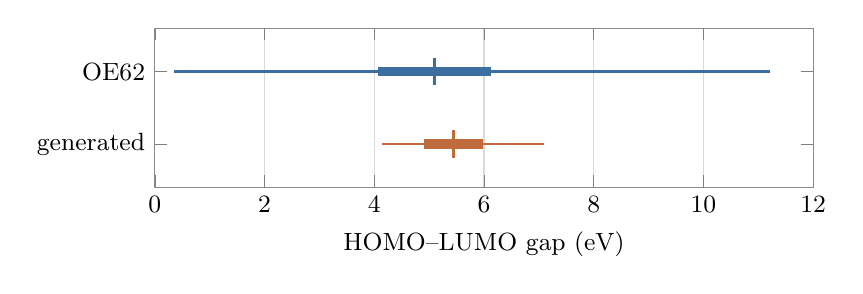
\begin{tikzpicture}
\begin{axis}[
  width=0.82\linewidth, height=3.6cm,
  xmin=0, xmax=12, ymin=0.4, ymax=2.6,
  xlabel={HOMO--LUMO gap (eV)}, label style={font=\small},
  ytick={1,2}, yticklabels={generated,OE62},
  yticklabel style={font=\small}, tick label style={font=\small},
  axis line style={cMuted}, xmajorgrids, grid style={cRule},
]
% OE62: min/max whisker, mean +- sigma box, mean tick
\addplot[cData,thick] coordinates {(0.343,2) (11.217,2)};
\addplot[cData,ultra thick,line width=3.4pt] coordinates {(4.063,2) (6.123,2)};
\addplot[only marks,mark=|,mark size=5pt,cData,line width=1.1pt]
  coordinates {(5.093,2)};
% generated
\addplot[cGen,thick] coordinates {(4.139,1) (7.089,1)};
\addplot[cGen,ultra thick,line width=3.4pt] coordinates {(4.908,1) (5.980,1)};
\addplot[only marks,mark=|,mark size=5pt,cGen,line width=1.1pt]
  coordinates {(5.444,1)};
\end{axis}
\end{tikzpicture}
\caption{Gap distributions: thin line spans observed
minimum to maximum, thick bar is $\mu\pm\sigma$, tick is the mean.
OE62 (\num{61489} molecules): $\mu=5.09$, $\sigma=1.03$, range
$[0.34,11.22]$. Unbiased generated samples (\num{241} molecules,
surrogate consensus): $\mu=5.44$, $\sigma=0.54$, range $[4.14,7.09]$.
The generator concentrates near the centre of the training distribution
and under-represents both tails.}
\label{fig:dist}
\end{figure}
% ---------------------------------------------------------------------

This has a direct consequence for any generate--filter--retrain loop:
the molecules available for selection occupy about half the width of the
data, and the unbiased minimum (\SI{4.14}{\electronvolt}) sits far above
OE62's own minimum (\SI{0.34}{\electronvolt}). Driving the distribution
down therefore means first recovering tail mass that the generator does
not produce spontaneously.

\subsection{Functional-group composition}

Figure~\ref{fig:enrich} compares functional-group frequencies in
unbiased samples against OE62. The generator over-produces alkenes by
$2.7\times$ and amines by $2.2\times$. We report only groups whose
expected count under the OE62 frequency exceeds $\approx$20 in our
sample; weaker apparent enrichments (e.g.\ iodine, five occurrences
against \num{2.5} expected) are not distinguishable from noise at this
sample size.

% ---------------------------------------------------------------------
\begin{figure}[t]
\centering
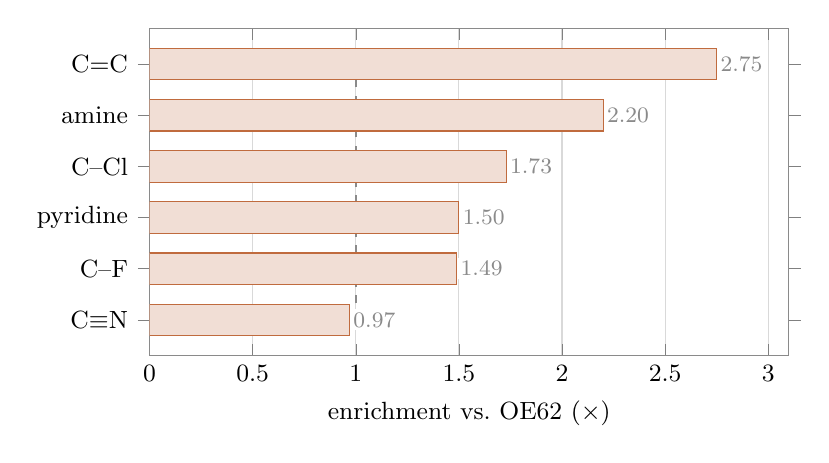
\begin{tikzpicture}
\begin{axis}[
  width=0.80\linewidth, height=4.4cm,
  xbar, y=6.5mm, bar width=4mm,
  xmin=0, xmax=3.1, xlabel={enrichment vs.\ OE62 ($\times$)},
  label style={font=\small},
  symbolic y coords={nitrile,halogenF,pyridine,halogenCl,amine,alkene},
  % ytick=data would order the ticks by the order the data appears, which
  % does not match the yticklabels list. Name the ticks explicitly.
  ytick={nitrile,halogenF,pyridine,halogenCl,amine,alkene},
  yticklabels={C$\equiv$N,C--F,pyridine,C--Cl,amine,C=C},
  yticklabel style={font=\small}, tick label style={font=\small},
  axis line style={cMuted}, xmajorgrids, grid style={cRule},
  enlarge y limits=0.14,
]
% Parity line first, so the bars and their labels sit on top of it.
\addplot[cMuted,dashed,thick,sharp plot,update limits=false,forget plot]
  coordinates {(1,nitrile) (1,alkene)};
% Value labels carry a white background so the 0.97 bar's label is not
% cut through by the parity line it sits beside.
\addplot[draw=cGen,fill=cGen!22,
  nodes near coords={%
    \pgfmathprintnumber[fixed,fixed zerofill,precision=2]{\pgfplotspointmeta}},
  nodes near coords style={font=\footnotesize,text=cMuted,
                           fill=white,inner sep=1.2pt}] coordinates {
  (2.75,alkene) (2.20,amine) (1.73,halogenCl)
  (1.50,pyridine) (1.49,halogenF) (0.97,nitrile)};
\end{axis}
\end{tikzpicture}
\caption{Functional-group enrichment in \num{145} unbiased generated
molecules relative to \num{10000} OE62 reference molecules. Dashed line
is parity. The nitrile group, the focus
of~\cite{westermayr2022}, is \emph{not} enriched before biasing
($0.97\times$), as expected.}
\label{fig:enrich}
\end{figure}
% ---------------------------------------------------------------------

The nitrile frequency in unbiased samples is
\num{0.0759} per molecule against OE62's \num{0.0781}
($0.97\times$). This is the correct null result: the cyano enrichment
of~\cite{westermayr2022} is a property of molecules \emph{selected for
small gaps}, not of unconditional samples, so it can only be tested
after several biasing iterations.

\subsection{Scope of the present study}

We report a single completed iteration. The \num{74} molecules selected
at iteration~0 span \SIrange{4.14}{5.18}{\electronvolt} in predicted
gap against a sampled mean of \SI{5.44}{\electronvolt}, and constitute
the training set for the first fine-tune. The multi-iteration
trajectory --- the displacement of the mean and the minimum across
successive iterations, and whether the count of usable molecules
degrades as the generator is fine-tuned on progressively smaller and
more selective training sets --- is the subject of ongoing work, and
we do not report it here. What the present results establish is the
baseline against which such a trajectory must be measured: the
unconditional distribution of Figure~\ref{fig:dist}, the
functional-group composition of Figure~\ref{fig:enrich}, and the
per-iteration yield of Table~\ref{tab:funnel-loop}.

% =====================================================================
\section{Discussion}
\label{sec:discussion}
% =====================================================================

\paragraph{Sampling cost is the binding constraint.} We measure
\SI{1.64}{\second} per molecule on a T4: the \num{3000} samples of
Table~\ref{tab:uncond} took \SI{82}{\minute} to draw.
Table~\ref{tab:cost} applies that rate to the protocol
of~\cite{westermayr2022}. A single one of their iterations would occupy
between \num{18} and \num{41} GPU-hours, so none of them fits in a
twelve-hour session, and the full protocol ranges from \num{128} to
\num{451} GPU-hours --- between four and fifteen weeks at the
\num{30} GPU-hours per week our environment provides.

\begin{table}[t]
\centering
\caption{The original protocol costed at our measured sampling rate of
\SI{1.64}{\second} per molecule. The published study reports
\numrange{40000}{90000} molecules per iteration over 7, 10 and 11
iterations for $\Delta E$, EA and IP respectively~\cite{westermayr2022}.}
\label{tab:cost}
\begin{tabular}{lrr}
\toprule
 & Molecules & GPU-hours at \SI{1.64}{\second}/mol. \\
\midrule
One iteration, lower bound  & \num{40000}   & \num{18.2} \\
One iteration, upper bound  & \num{90000}   & \num{41.0} \\
Full protocol, lower bound  & \num{280000}  & \num{128} \\
Full protocol, upper bound  & \num{990000}  & \num{451} \\
\midrule
\textbf{This work}          & \textbf{\num{3000}} & \textbf{\num{1.4}} \\
\bottomrule
\end{tabular}
\end{table}

 Our study therefore
operates at $\sim$1/100th of the original sampling scale, and that is a
direct consequence of the substitution: autoregressive generation costs
a few dozen cheap forward passes per molecule, whereas diffusion costs
hundreds of denoising steps over a fully connected graph. The
architectural advantages of diffusion are bought with sampling
throughput, and in a loop that depends on generating rare tail
molecules, throughput is exactly what is scarce.

\paragraph{The bottleneck is bond perception, not generation.} The
funnel of Table~\ref{tab:funnel-loop} loses more molecules to re-inferring
bonds from generated coordinates than to any other stage. EQGAT-diff
predicts bond orders natively; routing its output through a
coordinate-only format discards them and then fails to recover them for
roughly two thirds of the molecules the model itself judged valid. Preserving predicted bonds end to end is the single highest-value
change available, and it is available only because the generator was
swapped --- the original architecture had no bonds to preserve.

\paragraph{The surrogate is accurate on OE62 and unquantified on
samples.} Validation MAE of \SI{0.2262}{\electronvolt} is measured on
held-out OE62: equilibrium, crystal-derived DFT geometries. The loop
applies the surrogate to diffusion samples, which are off-equilibrium
and sometimes strained. The order-of-magnitude train--validation gap in
Figure~\ref{fig:oracle} indicates a model leaning on memorised
structure, and such models degrade fastest off-distribution. We
therefore treat \SI{0.2262}{\electronvolt} as a lower bound on selection
uncertainty, and mitigate with the two-surrogate agreement filter rather
than claiming the validation figure transfers.

\paragraph{Narrow unconditional distributions limit any such loop.}
Figure~\ref{fig:dist} shows the generator concentrating near the centre
of the training distribution. A loop that can only select from samples
it has already drawn is bounded by what the sampler produces
spontaneously; gradient-based guidance from a differentiable surrogate,
which steers trajectories rather than waiting for rare samples, is the
natural response and is supported by the diffusion
formulation~\cite{le2023} but not by the autoregressive one.

% =====================================================================
\section{Limitations}
% =====================================================================

\begin{itemize}
  \item \textbf{Property definition.} Our surrogate predicts the
        HOMO--LUMO gap as stored in OE62, a DFT quantity. The original
        study targets $GW$ fundamental gaps via $\Delta$-learning.
        Absolute values are therefore not comparable with theirs, and we
        report displacements rather than absolute targets. OE62's stored
        \texttt{homo} and \texttt{lumo} columns are internally
        consistent ($\mathrm{lumo}-\mathrm{homo}$ reproduces the stored
        gap exactly), but their absolute values sit $\approx$\num{5170}
        above physical orbital energies. Assuming typical organic
        HOMO and LUMO values, both columns imply the same offset to
        two decimals, which suggests a single additive constant of
        $\approx$\SI{5174.7}{\electronvolt}; we have not verified this
        against the published OE62 distributions. Ionisation potential
        and electron affinity are therefore accessible only up to an
        unknown constant, which permits relative but not absolute
        comparison.
  \item \textbf{No $GW$ verification.} \cite{westermayr2022} recompute
        selected molecules at the $G_0W_0$ level. Our property values are
        surrogate predictions, unverified by electronic-structure
        calculation.
  \item \textbf{Element coverage, and one finding it puts out of reach.}
        Bond perception removes all Se, As, Te and Li molecules, so the
        generator covers 12 of 16 elements. This costs more than a count.
        \cite{westermayr2022} report that molecules with small $\Delta E$
        show significantly increased sulfur \emph{and selenium} content,
        and attribute part of the gap reduction to O$\rightarrow$Se
        substitution --- on average \SI{1.1}{\electronvolt} when all
        oxygens are replaced. Because our preparation discards every
        selenium-containing molecule, that half of their chemical
        conclusion cannot be tested here at all; only the cyano finding
        is reachable.
  \item \textbf{Protocol deviation at the first iteration.}
        \cite{westermayr2022} seed the first biasing step with the
        extreme decile of OE62 itself ($\approx$\SI{10}{\percent} of the
        data), so the first fine-tune sees thousands of real molecules in
        the target range. Our iteration~0 instead selects from generated
        samples, giving a fine-tune set two orders of magnitude smaller.
  \item \textbf{No head-to-head generation metrics.}
        \cite{westermayr2022} do not report molecule or atom stability or
        a validity rate for G-SchNet on OE62, so the values in
        Table~\ref{tab:uncond} have no published counterpart to be
        compared against.
  \item \textbf{Scale.} $\sim$1/100th of the original sampling volume,
        with correspondingly weaker distributional statistics.
  \item \textbf{Descriptor substitutions.} We use Morgan fingerprints
        with PCA in place of SOAP, and RDKit's SA\_Score in place of
        SCScore. Five principal components explain only
        \SI{12.0}{\percent} of the variance in our fingerprint space,
        against the $>$\SI{98}{\percent} that \cite{westermayr2022}
        report for five components of their SOAP descriptors. Our
        embedding should therefore not be read as a faithful
        low-dimensional map of chemical space.
\end{itemize}


% =====================================================================
\section{Future Work}
% =====================================================================

Three extensions follow directly from the measurements above, in
increasing order of cost.

\subsubsection{Preserving predicted bonds.}
Section~\ref{sec:funnel} shows that routing generated structures through
a coordinate-only format and re-perceiving bonds discards roughly two
thirds of the molecules the generator itself judged valid. EQGAT-diff
emits bond types as part of its output; carrying them through to the
screening stage removes the stage entirely. This is an engineering
change rather than a research one, and it would raise the per-iteration
yield by a factor of about three at no sampling cost, which in turn
changes how much selection pressure the loop can afford.

\subsubsection{The cyano knock-out.}
\cite{westermayr2022} removed every C$\equiv$N bond from the training
data and found that G-SchNet reintroduced cyano groups when biased
towards small gaps, already after the first iteration. Repeating that
experiment with a diffusion generator asks whether the association is a
property of the chemistry or of the sampler. Our converter already
supports excluding molecules matching a SMARTS pattern, so the
experiment requires one additional training run on the knocked-out
corpus and one biasing run; both outcomes are informative, and a
negative result would be the more interesting of the two.

\subsubsection{Guidance instead of filtering.}
The combination of Figure~\ref{fig:dist} and
Table~\ref{tab:funnel-loop} makes an argument against the
generate--filter--retrain design for diffusion generators specifically.
The loop can only select from what the sampler happens to produce, the
sampler concentrates near the centre of the training distribution, and
sampling is expensive. Gradient-based guidance from a differentiable
surrogate steers trajectories towards the target during denoising
instead of waiting for rare tail samples to appear and then discarding
most of them, and is available for diffusion models but not for
autoregressive ones. Our surrogate reads coordinates and atomic numbers
only, so it is differentiable with respect to the coordinates the
diffusion process updates, and could be attached without
retraining.

% =====================================================================
\section{Conclusion}
% =====================================================================

Replacing an autoregressive generator with an equivariant diffusion
model inside a property-driven design loop is feasible. On
unconditional generation the diffusion model learns local chemistry
well --- \SI{97.9}{\percent} atom stability, small distributional
distances on bond lengths, valencies and charges --- with novelty of
\num{0.996} and uniqueness of \num{1.000}, and a molecule-level validity cost that the
error profile attributes to the twelve-element alphabet rather than to
geometry. The substitution also relocates the loop's
bottleneck. It is no longer the generator but the conversion of
generated coordinates back into bonded molecules --- a step the
diffusion model should render unnecessary, and would, if its predicted
bonds were preserved. Whether the chemical conclusion of the original
study survives the substitution is not settled here: that requires a
multi-iteration run, which remains ongoing work. What is settled is the
baseline it will be measured against --- an unconditional distribution
half as wide as the data, a selection yield of \num{74} molecules per
\num{3000} sampled, and no cyano enrichment before biasing, as there
should not be.

% =====================================================================


% =====================================================================
\section{Reproducibility}
% =====================================================================

All experiments ran on a single NVIDIA T4 in a publicly available cloud
notebook environment with a twelve-hour session limit, which is the
constraint behind the scale discussed in
Section~\ref{sec:discussion}. The generator is the reference
EQGAT-diff implementation with four small patches registering OE62 as a
dataset; the dataset class, the sharded bond-perception converter, the
surrogate trainer and the biasing loop are the only components we
wrote. The preparation pipeline is deterministic up to worker
scheduling, as the three-run spread in Section~\ref{sec:data}
indicates. Every count reported in Sections~\ref{sec:uncond}
and~\ref{sec:funnel} comes from a single generation run of \num{3000}
molecules, so the figures are mutually consistent rather than pooled
across runs.

\begin{credits}
\subsubsection{\ackname}
The authors thank the Department of Computer Science at Troy University
for computational support. Experiments were run on publicly available
cloud GPU resources.

\subsubsection{\discintname}
The authors have no competing interests to declare that are relevant to
the content of this article.
\end{credits}


% ---- Bibliography ----------------------------------------------------
% BibTeX users should specify bibliography style 'splncs04'.
% Verify venues, volumes and page numbers against the published
% versions before submission.
\begin{thebibliography}{8}

\bibitem{westermayr2022}
Westermayr, J., Gilkes, J., Barrett, R., Maurer, R.J.: High-throughput
property-driven generative design of functional organic molecules.
arXiv:2207.01476 (2022)

\bibitem{le2023}
Le, T., Cremer, J., No\'e, F., Clevert, D.-A., Sch\"utt, K.T.:
Navigating the design space of equivariant diffusion-based generative
models for de novo 3D molecule generation. arXiv:2309.17296 (2023)

\bibitem{stuke2020}
Stuke, A., Kunkel, C., Golze, D., Todorovi\'c, M., Margraf, J.T.,
Reuter, K., Rinke, P., Oberhofer, H.: Atomic structures and orbital
energies of 61,489 crystal-forming organic molecules. Sci. Data
\textbf{7}, 58 (2020)

\bibitem{gebauer2019}
Gebauer, N.W.A., Gastegger, M., Sch\"utt, K.T.: Symmetry-adapted
generation of 3D point sets for the targeted discovery of molecules.
In: Advances in Neural Information Processing Systems 32 (2019)

\bibitem{schutt2018}
Sch\"utt, K.T., Sauceda, H.E., Kindermans, P.-J., Tkatchenko, A.,
M\"uller, K.-R.: SchNet -- a deep learning architecture for molecules
and materials. J. Chem. Phys. \textbf{148}(24), 241722 (2018)

\bibitem{kim2015}
Kim, Y., Kim, W.Y.: Universal structure conversion method for organic
molecules: from atomic connectivity to three-dimensional geometry.
Bull. Korean Chem. Soc. \textbf{36}(7), 1769--1777 (2015)

\bibitem{ertl2009}
Ertl, P., Schuffenhauer, A.: Estimation of synthetic accessibility
score of drug-like molecules based on molecular complexity and fragment
contributions. J. Cheminform. \textbf{1}, 8 (2009)

\end{thebibliography}
\end{document}
